\newpage
\section{Reaktor}
\subsection{Luftesystem}
Når systemet er i lufting bygger blåsaren opp trykkluft til diffuserane i botn av tanken. 
Diffurserane er laga av ein membran med små hull som dannar bobler når lufta kjem i kontakt med avlaupsvatnet. Boblene tilfører oksygen til mikroorganismane i reaktorane. 
Lufting av reaktoren er også med på å blande avlaupsvatnet og forhindrar at det aktive slammet legger seg i botn på reaktoren i reaksjonsfasen.

Dersom membranen på diffuseren strekkast ut eller blir ujamn kan dette føre til tap av effektivitet på lufting i tanken.

Luftesystemet er bygd opp av fleire diffusere som dekker mesteparten av botnarealet i reaktoren.

\begin{figure}[htbp]
    \centering
    \begin{subfigure}[b]{0.3\textwidth}
        \centering
        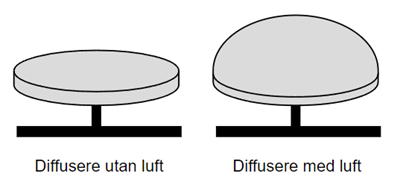
\includegraphics[width=1\textwidth]{Figurar/DiffusereMedOgUtanLuft.png}
        \caption{Diffuser oppsett i reaktor}\label{fig:subfig1}
    \end{subfigure}
    \hfill
    \begin{subfigure}[b]{0.3\textwidth}
        \centering
        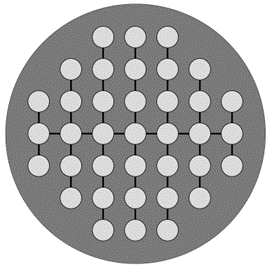
\includegraphics[width=1\textwidth]{Figurar/DiffuserFraTopp.png}
        \caption{Illustrasjon diffusere}\label{fig:subfig2}
    \end{subfigure}
    \caption{Illustrasjon av diffusere}\label{fig:Illustrasjon-Diffuser}
\end{figure}

\newpage
\subsection{Reaktor-soner}

\begin{figure}[htbp]
    \centering
    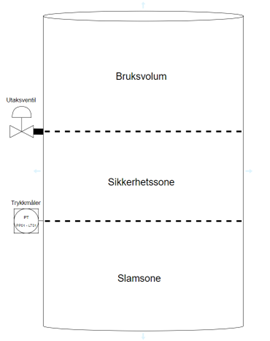
\includegraphics[width=0.3\textwidth]{Figurar/Reaktorsoner.png}
    \caption{Illustrasjon reaktorsoner}\label{fig:reaktorsoner}
\end{figure}

\textbf{Bruksvolum} \newline
Bruksvolumet er den aktive delen av tanken som fyllast ved kvar innpumpingsekvens

\textbf{Slamsona} \newline
Slamsona er den delen av tanken som er under utløpet, fråtrekket sikkerheitssona. Her ligger det aktive slammet.

\textbf{Sikkerheitssona} \newline
Den tredje sonen er sonen mellom bruksvolumet og slamsonen. Den er til for å ta hand om varierande sedimenteringseigenskapar og overskuddsslam.

I reaksjonssekvensen blandast desse sonene ved lufting av reaktoren. I sedimenteringssekvensen vil desse sonene komme tilbake og det reinsa avlaupsvatnet vil okkupere bruksvolumsona og kan drenerast til resipient.
